% Brief introduction with 
\Gls{pet} makes use of positron-emitting radionuclides for the study of biochemical and physiological processes \textit{in vivo}. The molecules of interest for the processes under study are labelled with a radionuclide and then introduced in the body. The PET imaging system provides information about the distribution of the labelled molecules \textit{in vivo} over time and can be used to deduce information about the underlying process kinetics. 

\section{Principles of pharmacokinetic modelling}
Pharmacokinetics refers to the study of absorption, distribution, metabolism and excretion of drugs in living systems. The study of pharmacokinetics is based on measurements of the concentration of drugs and their metabolites in tissues over time. Pharmacokinetic models describe the transport and binding rates of tracer from local concentration differences across boundaries, that can be either physical (such as a membrane or an organ outline) or conceptual boundaries as for example between bound and unbound tracer. These boundaries define separate compartments with distinct activity concentration which form the basis of pharmacokinetic models, also referred to as compartmental models.
%There are three assumptions are made for compartmental modelling to be valid:
%The first is the tracer assumption which requires that the presence of the tracer in PET studies is not influencing the physiological processes and molecular interactions. This is the case in most PET studies as the specific activity of the tracer (Activity/tracer concentration) is kept low. The second assumption is that the physiological processes and molecular interactions are in constant state during the duration of the PET study. The third and final assumption is that tracer is homogeneously distributed within each compartment. 

The three key assumptions underlying compartmental modelling are:
\begin{itemize}
\item The concentration of the PET tracer is not high enough to influence the physiological processes and endogenous molecular interactions under study.
\item That all physiological processes and interactions are in constant state for the duration of the PET study.
\item The assumption that tracer concentration is instantly uniform in all compartments of the model.
\end{itemize}

By common convention in pharmacokinetic modelling, the first compartment is the arterial plasma pool from where the tracer distributes to tissues. The concentration of tracer in the arterial plasma $C_P(t)$ over time $t$ is measured or deduced from population studies and applied to the model, as an input function that powers the system.
If the tracer is metabolised during the study, this process needs to be modelled using metabolite measurements. Only the concentration of parent tracer can be used as input function in quantitative analysis of the tracer kinetics.
By convention in dynamic PET studies conducted under a single session, the time point $t_0=0$ is set to be the tracer injection time. \\
Compartmental models behave according to a set of first-order ordinary differential equations, which means that the change of concentration in one compartment is a linear function of the concentrations of all compartments. This linearity establishes that the measured tissue activity concentration will be the convolution of the input function with the impulse response function (IRF) of the system, which is described by the compartmental model and its parameters.
As such the tissue activity concentration $C_T(t)$ can be modelled as
\begin{equation}
 C_T(t) = C_P(t) \ast \textrm{IRF}(t)  \\ , \\ 
\end{equation}
where $\ast$ is the convolution operator. 

When a measurement of activity concentration is made with \gls{pet}, the measurement will include the underlying tissue activity and activity from the intravascular blood in this tissue. The proportion of tissue volume occupied by intravascular blood $V_B$ is commonly referred to as blood fraction.The measured activity concentration $C_{PET}$ can be expressed as
\begin{equation}
{C_{PET}}(t)  = (1-V_{B}){C_{T}}(t) + V_{B}C_{B}(t) \\ , \\
\label{eqn:CPET}
\end{equation}
where $C_{B}$ is the total blood activity concentration.
Measurements of the %metabolite corrected
arterial plasma to total blood ratio can be made to relate between $C_{B}(t)$ and $C_P(t)$. 
For the tracers of interest in this PhD project, the ratio of the two concentrations is assumed to be constant with time and to be $C_{B}(t) = r C_{P}(t)$. 

\section{One-tissue compartment model}
As the simplest model, the one-tissue compartment model (1TCM) can be described using two constant rates for the input and output of tracer from the tissue, $K_1$ and $k_2$ respectively. A representation can be seen in figure~\ref{fig:1_2TCM}.

\begin{figure}[ht]
	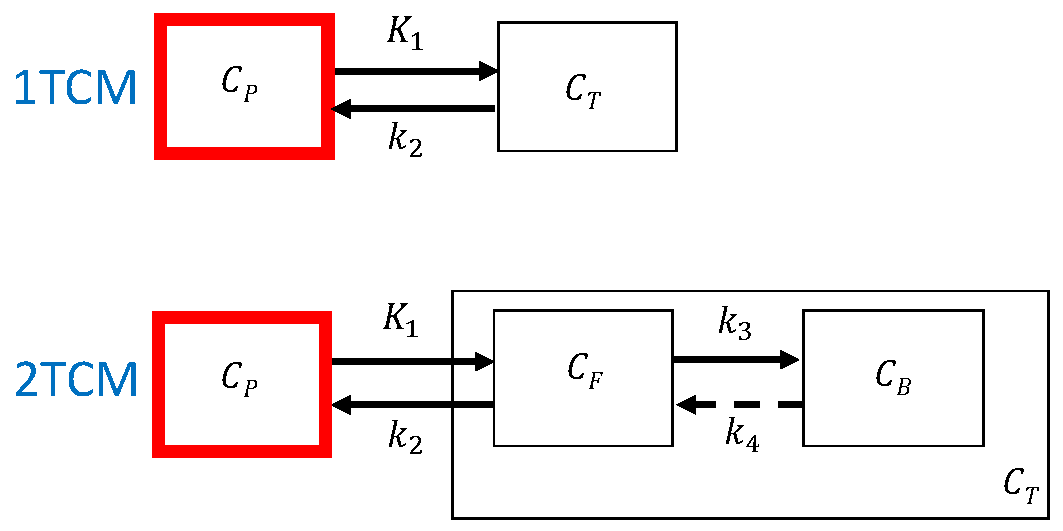
\includegraphics[width=0.8\textwidth]{2_Theory_Methods/figures/TissueCompartmentModels.pdf}
	\centering
	\caption{Representation of compartments and exchanges rates for 1TCM (top) and 2TCM (bottom)}
	\centering
	\label{fig:1_2TCM}
\end{figure}

The rate of change of the activity concentration in tissue $C_T$ will depend on the metabolite corrected arterial plasma input function $C_P$ and the activity concentration in tissue, described by the differential equation~\ref{eqn:1TCM_Diff}.

\begin{equation}
  \frac{\mathrm d C_T(t)}{\mathrm d t} = K_1 C_P(t) - k_2 C_T(t)
  \label{eqn:1TCM_Diff}
\end{equation}
\begin{equation}
   C_T(t) = K_1 e^{-k_2 t} \ast C_P(t) 
  \label{eqn:1TCM}
\end{equation}
\begin{equation}
   C_{PET}(t) =   K_1 e^{-k_2 t} \ast C_P(t) (1-V_B) + C_B(t) V_B
  \label{eqn:1TCM_CPET}
\end{equation}

Equation \ref{eqn:1TCM} is the solution of the differential equation \ref{eqn:1TCM_Diff}, which becomes \ref{eqn:1TCM_CPET} for the PET measurement that includes the fractional blood volume. %In equation \ref{eqn:1TCM_CPET} it is important to note that the blood fraction is related to the whole blood activity concentration $C_B$ , rather than the metabolite corrected activity concentration $C_A$. When the tracer metabolic activity is negligible and under the assumption of negligible tracer delay and diffusion from arterial to venous blood TACs, the two concentrations ($C_A = C_B$) can be set equal in favour if simplified models and estimations. 

\section{Two-tissue compartment model}
The two-tissue compartment model (2TCM) is a commonly used model as it describes the behaviour of ${}^{18}F$-Fluorodeoxyglucose (${}^{18}\mathrm{F}$-FDG), which is commonly used tracer in clinical and research PET protocols. The separation into two tissue compartments is made to distinguish between free and trapped (bound) tracer, represented as $C_F(t)$ and $C_B(t)$ respectively, with the trapping caused by the tracer being metabolised in the cells by mitochondria. The set of differential equations describing the 2TCM is shown in equations~\ref{eqn:2TCM_Diff}.

\begin{subequations}
\begin{align}
%C_{PET} = (C_F + C_B)(1-V_B) + V_B C_A \\
\frac{d}{dt}C_F(t) = K_1 C_A(t) - (k_2 + k_3)C_F(t) + k_4 C_B(t) \\ 
\frac{d}{dt}C_B(t) = k_3 C_F(t) - k_4 C_B(t)  
\end{align}
\label{eqn:2TCM_Diff}
\end{subequations}

The pathway of tracer from the trapped to the free state, via the process of dephosphorylation, is commonly considered negligible for the duration of common PET studies. With the assumption of $k_4=0$ the two differential equations in \ref{eqn:2TCM_Diff} simplify to the system \ref{eqn:2TCM_Diff_k4=0} which when solved results in equation \ref{eqn:2TCM}. 

\begin{subequations}
\begin{align}
\frac{d}{dt}C_F(t) = K_1 C_A(t) - (k_2 + k_3)C_F(t) \\ 
\frac{d}{dt}C_B(t) = k_3 C_F(t)  
\end{align}
\label{eqn:2TCM_Diff_k4=0}
\end{subequations}
%
\begin{equation}
C_T(t) =  C_F(t) + C_B(t) = K_1 ( e^{-(k_2+k_3)t} + \frac{k_3}{k_2+k_3}(1-e^{-(k_2+k_3)t})) \ast C_P(t)   
\label{eqn:2TCM}
\end{equation}

The parameters $K_1$, $k_2$ and $k_3$, which are referred to as micro-parameters, can be estimated by fitting equation~\ref{eqn:2TCM} on measured \gls{tac} data. 

A parameter of interest for clinical studies is the influx rate constant $K_i$, given by equation~\ref{eqn:FDG_Ki}. This is considered as a macro-parameter of the system and can be understood as the proportion of flux $K_1$ that results in trapped tracer.

\begin{equation}
K_i = \frac{K_1 k_3}{k_2+k_3} . 
\label{eqn:FDG_Ki}
\end{equation}

The influx of FDG is proportional to the influx of glucose, also referred as the glucose metabolic rate $MR_{glu}$. The proportionality constant is called the lumped constant $LC$ and along with the concentration of blood glucise $C_{P}^{glu}$ can be used to express
\begin{equation}
MR_{glu} = K_i \Big(\frac{C_{P}^{glu}}{LC}\Big)
\label{eqn:MR_glu}
\end{equation}


\section{Gjedde-Patlak linearisation method}
Direction estimation of model micro-parameters, such as those of equation~\ref{eqn:2TCM}, requires non-linear fitting optimization procedures. These are commonly time consuming and their estimations are heavily susceptible to noise.
For parametric imaging, where the model estimation has to be performed for every voxel of the image, estimation of micro-parameters is commonly avoided due to the poor statistics and high noise associated with \gls{tac} measurements at the voxel level. 
Linearisation methods allow for transformation of the measured data, to enable use of linear least-square fitting procedures for estimation of model macro-parameters, under certain assumptions. Furthermore, these methods reduce the number of parameters to be estimated, thus reducing the variability of estimates and sensitivity to noise. 

With the assumption of irreversible tracer behaviour the Gjedde-Patlak method has been developed, described by Gjedde~\cite{Gjedde1982} and Patlak \textit{et al.}~\cite{Patlak1985}. The proposed transformation is

\begin{equation}
\label{eqn:PatlakModel}
\frac{C_{T}(t)}{C_{P}(t)} = K_i \frac{\int_{0}^{t} C_{P}(\tau) d\tau}{ C_{P}(t)} + V_{\alpha}   \ , \;  t>t_{ss} \ ,
\end{equation}

where $K_i$ is the steady state trapping rate and $V_{\alpha}$ the apparent volume of distribution. The transformation is valid for time points $t$ after steady state conditions are achieved at time $t_{ss}$. Steady state conditions are achieved when the reversible compartments are in steady-state equilibrium with the plasma blood compartment. 

The Gjedde-Patlak linearisation method referred to simpler as \textit{Patlak model}, is commonly used with the 2TCM model for FDG, under the assumption of $k_4=0$. In this case, the Patlak model parameters can be related to micro-parameters using equation~\ref{eqn:FDG_Ki} and 

\begin{equation} 
V_{\alpha}  = \frac{K_1 k_2}{(k_2+k_3)^2} \\ . \\ 
\end{equation}

%For a PET measurement the observed activity $C_{PET}(t)$ described by equation~\ref{eqn:CPET}.
With the assumption of $C_{B}(t) = r C_{P}(t)$, we can substitute equation~\ref{eqn:PatlakModel} into equation~\ref{eqn:CPET} and describe the observed activity $C_{PET}(t)$ using the Patlak model as

\begin{equation} 
\frac{C_{PET}(t)}{C_{P}(t)} = \underbrace{(1-V_{B})K_i}_{\theta_1} \frac{\int_{0}^{t} C_{P}(\tau) d\tau}{ C_{P}(t)} +  (\underbrace{V_{\alpha}(1-V_{B})+r V_{B}}_{\theta_2}) \\ , \\
\label{eqn:PatlakCPET}
\end{equation}

where the Patlak slope $\theta_1$ and the Patlak intercept $\theta_2$ are the model parameters that can be estimated from TAC measurements of ${C_{PET}}(t)$. 

%It is important to note a limitation of the Patlak model, which  that the estimated $K_i$ from the Patlak slope $\theta_1$ is susceptible to systematic errors in its estimation and can deviate from the true underlying $K_i (= \frac{K_1 k_3}{k_2+k_3})$.
A limitation in the use of the Patlak model using equation~\ref{eqn:PatlakCPET} is that $V_B$ is not necessarily known a priori and Patlak analysis can not distinguish between $K_i$ and $(1-V_B)$. In many applications, $V_B$ is assumed to be small ($\leq$0.05) and neglected, but it can be a cause for systematic errors. 
In the applications of the Patlak model in this project, we will refer to the slope $\theta_1$ as the Patlak $K_i$ value, which is the value of interest that is commonly used in practice with Patlak analysis.


\section{Spectral analysis method}
The Spectral analysis method was originally introduced by Cunningham et al. \cite{Cunningham1993}. The method is based on the general form of the solutions of compartmental models and describes the generic behaviour of any compartmental system as a positively weighted sum of decaying exponential functions with decay rates $\beta$ which describe the exchange between compartments, convolved with an input function. 

The spectral analysis model for $C_T(t)$ can be expressed using M functions as

\begin{equation} 
\label{eqn:SpectralModel}
C_{T}(t)  =  \sum_{b=0}^{M-1} {\phi_b}  e^{-\beta_b t} \ast C_P(t)   \\ , \\
\end{equation}

where $\phi_b$ are the model coefficients (constrained to positive values) for the exponential functions with decay rates $\beta_b$ that describe the exchange between compartments. 

The advantage of this methodology is that it can be used to fit on \gls{tac} data, with few assumptions on the underlying kinetics. Additionally, it can be used to deduce information of the underlying kinetics using the basis pursuit strategy proposed by Gunn \textit{et al.}~\cite{Gunn2002}.
Macro-parameters of the underlying model can also be deduced using the spectral analysis fitted model. Tracer delivery to tissue $K_1$ can be estimated directly with
\begin{equation} 
\label{eqn:SpectralModel_K1}
K_1  =  \sum_{b=0}^{M-1} {\phi_b}   \\ . \\
\end{equation}

For reversible kinetics, the parameters can be used to deduce the volume of distribution $V_D$ as
\begin{equation} 
\label{eqn:SpectralModel_VD}
V_D  =  \sum_{b=0}^{M-1} \frac{\phi_b}{\beta_b}   \\ . \\
\end{equation}

For irreversible kinetics, a parameter of the model is used to account for the trapping rate $K_i$. In this work we use parameter ${\phi_0}$ to describe irreversible trapping, with its respective exponential decay rate set to zero ${\beta_0} = 0 $. With this assumption the model becomes

\begin{equation} 
\label{eqn:SpectralModel_Complete}
C_{T}(t)  = \phi_0 \ast C_P(t) + \sum_{b=1}^{M-1} {\phi_b}  e^{-\beta_b t} \ast C_P(t)  \\ , \\
\end{equation}

for which $K_i = {\phi_0}$. 

Finally, to model the observed activity $C_{PET}(t)$ using the spectral analysis model, we can substitute equation~\ref{eqn:SpectralModel} into equation~\ref{eqn:CPET} and assume again that $C_{B}(t) = r C_{P}(t)$ to get

\begin{equation} 
{C_{PET}}(t)  = (1-V_{B}) \sum_{b=0}^{M-1} {\phi_b}  e^{-\beta_b t} \ast C_P(t) + r V_{B}  C_P(t)   \\ . \\
\label{eqn:SpectralCPET}
\end{equation}

If we account for the parameter $(1-V_{B})$ into the weights $\phi_b$, the equation can be written in short as 

\begin{equation} 
{C_{PET}}(t)  = \sum_{b=0}^{M} {\phi_b} e^{-\beta_b t} \ast C_P(t)   \\ , \\
\label{eqn:SpectralCPET_short}
\end{equation}

for which $\beta_M \xrightarrow[]{}\infty$ and $\phi_M = r V_{B}$. 
When fitted on measured ${C_{PET}}(t)$ data, the spectral model in equation~\ref{eqn:SpectralCPET_short} can be used to deduce $K_1$, and either $V_D$ or $K_i$ respectively for reversible or irreversible tracers behaviour, using

\begin{subequations}
\label{eqn:AllSpectralEqns}
\begin{align}
K_1 = \frac{\sum_{b=0}^{M-1} {\phi_b}}{1-{V_{B}}}   \\  
V_D = \sum_{b=0}^{M-1} \frac {\phi_b}{\beta_b (1-V_{B})} \\
K_i = \frac{\phi_0}{1-V_{B}} .
\end{align}
\label{eqn:SpectralCPET_AllEquations}
\end{subequations}
%
\subsection{Choice of spectral rates}
%
On equation~\ref{eqn:SpectralCPET_short} the spectral rates $\beta_1 ... \beta_{M-1}$ are used to describe the exchange between compartments. These are set to cover the range of expected underlying kinetics and are commonly logarithmically spaced within that range~\cite{Gunn2002}.
As a rule of thumb, the lower limit of the range can be set to $\beta_1 = 1/(3 T_{end})$ where $T_{end}$ is the total time of the PET study, and the upper limit of the range can be set to $\beta_{M-1} = 3/T_{in}$ where $T_{in}$ is the duration of the first frame of the study~\cite{Veronese2016}.

In spectral analysis, the number of the spectral parameters used is empirically set in the 10$^2$ order of magnitude. This relatively large number allows for clear separation of the underlying exchange rates, for deduction of models of the underlying behaviour. 
For use with dynamic reconstruction a smaller number of parameters is used, ideally less than the number of time bins (frames) of the data, which is still adequate to model the PET measurements while maintaining low image noise.

\section{IsotoPK pharmacological study}
Traditionally it has been assumed that passive diffusion is the main mechanism controlling drug delivery to tissues. 
But it is now recognised that the presence of membrane transporters at blood-tissue interfaces suggests that transporters also play an important role in drug pharmacokinetics. DWB imaging studies can play an important role in the study of transporter distribution and function in regards to drug delivery to tissues over the body~\cite{Marie2017}. 
To this purpose, a novel PET tracer has been developed using Glyburide (glibenclamide, GLB) labelled with $^{11}$C. Glyburide is a drug used for treatment of diabetes and targets many transporters of the Solute Carrier O (SLCO) family~\cite{Tournier2013,Caille2020}. Preliminary pre-clinical studies have indicated that these transporters are expressed mainly in the liver and the kidneys~\cite{Tournier2013}.

A first in man study, named \textit{IsotoPK}, was designed and is being conducted in our centre for the study of the distribution of these transporters in healthy volunteers~\cite{Marie2019}.
The study is conducted on the Signa PET/MR, using a Dynamic Whole Body (DWB) acquisition protocol, with two acquisitions per volunteer to study the distribution without and with the administration of an inhibitor substance prior to PET imaging.
Arterial blood samples for deduction of an input function and metabolite analysis are collected manually during the duration of each scan. 

Data from this study are presented in chapter~\ref{Chap3_3:IsotoPK}, showing examples of distribution of the tracer on an example volunteer. The use of the data in this project was made with a focus on methodological aspects for whole-body parametric imaging, but the developed methodology will be used in the future after all volunteer data have been collected to evaluate its findings.
Initial results on three volunteers have shown that Glyburide is very slowly metabolised and therefore did not require metabolites to be accounted for in PET analysis, since their impact on PET quantification would be minimal. Findings also showed strong binding of tracer with plasma ($\geq$ 90\%).
Predominant uptake of the tracer was seen in the liver and also the kidneys. Lower uptake was observed in the spleen, the aorta wall and the pancreas. At all other tissues, no strong tracer uptake was seen.

Data coming from this protocol were used in this thesis. The IsotoPK study was the first DWB protocol to be conducted on the Signa PET/MR. 

\subsection{PET analysis in the liver}
\label{liver_PV_theory}
One of the unique characteristics of the liver, in regards to pharmacokinetic modelling, is that it is supplied with blood via two routes. The hepatic artery (HA) accounts for approximately 25\% of the blood supply in the liver, while the portal vein (PV) accounts for the rest 75\%~\cite{Winterdahl2011}. The portal vein delivers blood that has been filtered mainly by the gastrointestinal tract, a process that alters the characteristics of the portal vein input function. 
Studies on pigs and non-invasive studies on humans have produced methods to model the PV input function as a dispersion of the arterial input function~\cite{Kudomi2008}, which can be modelled using 

\begin{equation} 
{C_{PV}}(t)  = {k_g} e^{-k_g t} \ast C_P(t)   \\ . \\
\label{eqn:PortalVein}
\end{equation}

With knowledge of the $k_g$ dispersion value and ratio between PV and HA input, the liver input function ${C_{H}}(t)$ can be then modelled as

\begin{equation} 
{C_{H}}(t)  = 0.75 \cdot C_{PV}(t) + 0.25 \cdot C_{P}(t)  \\ . \\
\label{eqn:HepaticInput}
\end{equation}

An toy example demonstration of the two components of ${C_{H}}(t)$ is shown in figure~\ref{fig_2_2:LiverDualInputFunction}.

\begin{figure} [h!]
\centering
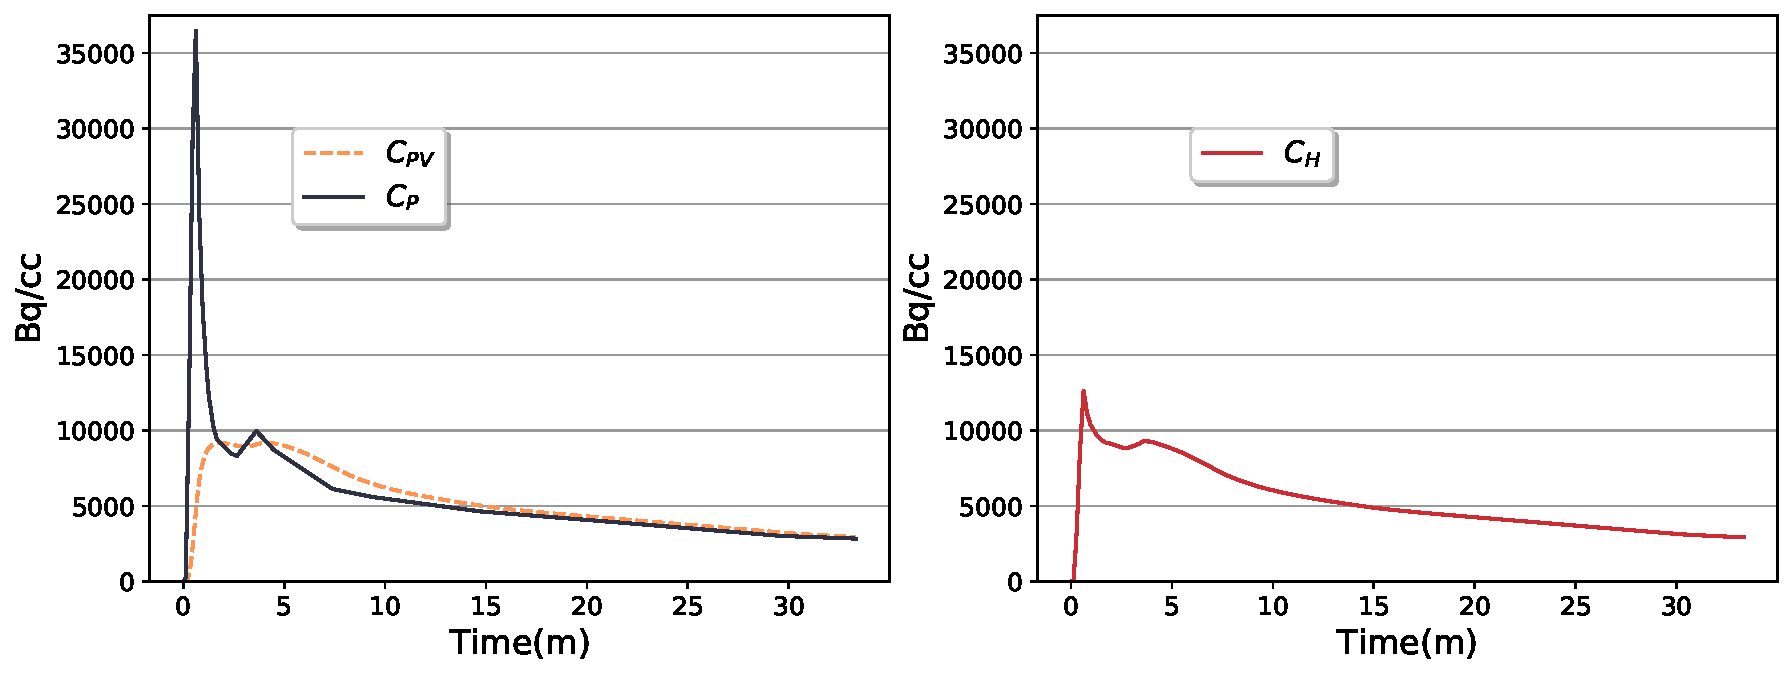
\includegraphics[scale=0.53,angle=0]{2_Theory_Methods/figures/2_2_LiverDualInputFunction.pdf}
\caption[Example measured arterial input function $C_{P}(t)$ and modelled PV input function (using $k_g$=0.5 min$^{-1}$) (left). Combination of arterial and PV input function to provide ${C_{H}}(t)$, assuming a 25/75 ratio (right).]{Example measured arterial input function $C_{P}(t)$ and modelled PV input function (using $k_g$=0.5 min$^{-1}$~\cite{Kudomi2008}) (left). Combination of arterial and PV input function to provide ${C_{H}}(t)$, assuming a 25/75 ratio (right).} 
\label{fig_2_2:LiverDualInputFunction}
\end{figure} 

The use of imaging information for non-invasive estimation of the portal vein input function and their effects in pharmacokinetic model estimates over the liver is an active area of research~\cite{Wang2018,HernandezLozano2019,Wang2021} with no standardised and widely accepted practices established yet. Further interest and research into DWB imaging is expected to address these issues for accurate WB parametric imaging that accurately accounts for the liner dual input model.  

%\subsection{Tracer redistribution}
%Another aspect 

